\namedchapter[Daniel Łukwiński]{Algorytm przetwarzania obrazu}
Zadanie, jakie miał realizować robot polegało na namierzeniu oraz śledzeniu celu w swoim otoczeniu. Założeniem było także to, aby algorytm robota potrafił znajdować cel przy zróżnicowanym oświetleniu oraz na różnej odległości (tj. niezależnie od jego rozmiaru na obrazie). Ważne było także, aby celem mógł być każdy obiekt spełniający podstawowe warunki koloru i kształtu. Algorytm przetwarzania i analizy obrazu ma więc za zadanie poszukiwać na dostarczanym przez kamerę obrazie celu i uzyskiwane w ten sposób informacje przesyłać do części programu odpowiedzialnej za sterowanie robotem.

\namedsection{OpenCV}
OpenCV jest biblioteką służącą do wszechstronnej obróbki obrazu, wydaną na licencji BSD (\textit{Berkeley Software Distribution}), będącej zgodną z zasadami wolnego oprogramowania. Została ona napisana w C oraz C++, jednak możliwe jest je wykorzystywanie także w języku \textit{Python} oraz \textit{Java}. Wspiera ona takie systemy operacyjne jak: \textit{Windows, Linux, Mac OS, iOS} oraz \textit{Android}. Posiada ona moduły służące do pracy tak z obrazem dwuwymiarowym, jak i trójwymiarowym. Ponadto zawiera szereg modułów, służących między innymi do rozpoznawania twarzy, gestów czy systemów uczących się (ang. \textit{machine learning}).

O jej wykorzystaniu, poza darmową licencją, zdecydowała optymalizacja zastosowanych rozwiązań oraz mnogość funkcji, spełniających większość zadań związanych z analizą obrazu. Wykorzystywana w projekcie wersja nosi oznaczenie 3.0.0 i została opublikowana 4 czerwca 2015 roku. W przedstawianym algorytmie wykorzystywane są trzy moduły z tej biblioteki:
\begin{itemize}
\item \texttt{core.hpp} - zawiera podstawowe klasy oraz funkcje związane z pracą na obrazach dwuwymiarowych;
\item \texttt{imgproc.hpp} - zawiera bardziej zaawansowane funkcje służące to przetwarzania obrazów, np.: filtrację obrazu czy progowanie;
\item \texttt{highgui.hpp} - w tym pliku znajdują się funkcje związane z interface'm programu, które zostały wykorzystane jedynie na etapie tworzenia algorytmu, do testowania jego efektów efektów (wyświetlenie obrazu, odczyt oraz zapis do pliku).
\end{itemize}

\namedsection{Inicjalizacja}
Działający na Raspberry Pi program składa się z dwóch części. Pierwsza z nich jest odpowiedzialna za inicjalizację sprzętowych generatorów sygnału PWM na Raspberry oraz łączenie się z kamerą oraz rozpoczęcie jej pracy z ustalonymi parametrami.

Inicjalizacja sygnałów PWM na Raspberry jest wykonywana z wykorzystaniem biblioteki \textit{wiringPi}. Jest to napisana w języku C biblioteka obsługująca piny GPIO mini komputera Raspberry Pi. Została ona wydana na licencji \textit{GNU LGPLv3}, umożliwiającej darmowy dostęp dla wszystkich zainteresowanych użytkowników. Pierwszym krokiem inicjalizacji sygnałów PWM jest wywołanie funkcji \texttt{int wiringPiSetupGpio()}. Znajdują się w niej deklaracje niezbędne do poprawnej pracy z biblioteką. Odpowiada ona także za umożliwienie bezpośredniego dostępu do pinów GPIO Raspberry. Wartością zwracaną przez tą funkcję jest kod, informujący o poprawności wywołania. Jego wartość równa -1 oznacza błąd uniemożliwiający dalszą prawidłową pracę. Następnie należy wywołać funkcję \textit{void pinMode (int pin, int mode)}, której zadaniem jest ustawienie jednego z pinów GPIO Rasppbery w odpowiedni tryb: wejścia, wyjścia, wyjścia zegara lub wyjścia sygnału PWM. W tym przypadku koniecznie jest ustawienie pinów numer 18 oraz 19 jako wyjścia sygnału PWM. Kolejną wywoływaną funkcją z tej biblioteki jest void \texttt{pwmSetMode(int mode)}. Ma ona za zadanie ustalić w którym z dwóch trybów ma pracować generator sygnału PWM: \textit{mark:space} lub \textit{balanced}. Pierwszy z nich jest klasycznym sygnałem PWM, w którym okres sygnału jest równy całemu cyklowi pracy jego licznika. W drugim wartość wypełnienia jest równomiernie rozłożona na cykl liczniki, przez wyjściowa częstotliwość sygnału jest dużo większa. W zastosowanym algorytmie wykorzystany został pierwszy tryb, gdyż dużo lepiej nadaje się on do sterowania serwomechanizmów. Kolejne dwa niezbędne do ustawienia parametry to zakres licznika oraz preskaler zegara. Wykorzystuje się do tego dwie funkcje: \texttt{void pwmSetRange (unsigned int range)} oraz \texttt{void pwmSetClock (int divisor)}. Wpływ tych dwóch parametrów przedstawia wzór
\begin{equation}
f_{PWM} = \frac{f_{count}}{range} = \frac{f}{(divisor * range)}
\label{eq:hard_pwm}
\end{equation}
gdzie:
\begin{equationDescriptor}
\EQDitem{$f_{PWM}$}{częstotliwość sygnału PWM [$Hz$],}
\EQDitem{$f_{count}$}{częstotliwość pracy licznika [$Hz$],}
\EQDitem{$f$}{częstotliwość zegara bazowego [$Hz$],}
\EQDitem{$divisor$}{Wartość preskalera,}
\EQDitem{$range$}{Zasięg licznika, }
\end{equationDescriptor}
W przypadku zastosowanych serw wymagane $f_{PWM}$ wynosi 50 $Hz$, a $f$ dla Raspberry Pi to 19.2 $MHz$. Przedstawiony wcześniej wzór przyjmuje więc postać:
\begin{equation}
50 Hz = \frac{19.2 MHz}{(divisor * range)}
\label{eq:hard_pwmN}
\end{equation}
Widać więc jasno, że wartość preskalera oraz zasięg liczniki są ze sobą powiązane i muszą być ustawiane wspólnie, a wartość ich iloczynu wynosi:
\begin{equation}
(divisor * range) = \frac{19.2 MHz}{50 Hz} = 384000
\label{eq:range_x_presc}
\end{equation}
O dokładności sterowania serwomechanizmem decyduje właśnie wartość zasięgu licznika służącego do generowania sygnału PWM. Wspomniane wcześniej funkcje z biblioteki \textit{WiringPi} służące do ustawiania tych dwóch parametrów przyjmują tylko wartości całkowite, więc wybierany zasięg licznika powinien być dzielnikiem liczby $384000$. Wartość zasięgu ustawiono więc na poziomie 6000, co zapewnia wystarczającą dokładność pracy serwomechanizmu, a to z kolei pociągnęło za sobą ustawienie preskalera zegara na 64. Ostatecznie blok kodu odpowiedzialny na inicjalizację sprzętowego generatora sygnału PWM w Raspberry Pi za pomocą biblioteki \textit{WiringPi} przyjmuje postać:
\begin{lstlisting}
if (wiringPiSetupGpio() != -1)
{
	pinMode(18,PWM_OUTPUT);
	pinMode(19,PWM_OUTPUT);
	pwmSetMode(PWM_MODE_MS);
	pwmSetRange(6000);
	pwmSetClock(64)
}
else
{
	return -1;
}
\end{lstlisting}

Drugą rzeczą, obok sygnału PWM, wymagającą inicjalizacji na początku pracy programu jest kamera. Do jej obsługi wykorzystana została biblioteka \textit{RaspiCamCV}, udostępniana na zasadach wolnego oprogramowania. Została ona wybrana, ponieważ zapewnia podstawową obsługę dedykowanej kamery Raspberry we współpracy z biblioteką \textit{OpenCV}. Z jej wykorzystaniem możliwe jest pobieranie rejestrowanych obrazów bezpośrednio w formacie umożliwiającym dalszą edycję za pomocą funkcji \textit{OpenCV}. Pierwszy etapem pracy z dedykowaną kamerą, z wykorzystaniem biblioteki \textit{RaspiCamCV} jest utworzenie danych konfiguracyjnych, które posłużą do pracy z kamery. Podstawową ustawieniem, które należy wybrać jest rozdzielczość w jakiej będą rejestrowane obrazy. Jest to o tyle istotne, że podstawowym ograniczeniem w pracach nad algorytmem wykrywającym cel był fakt, że wyniki jego pracy miały na bieżąco sterować ruchami pojazd, przy ograniczonej mocy obliczeniowej platformy Raspberry Pi. Podstawowym ograniczeniem, które spowodowały te warunki, była rozdzielczość analizowanego obrazu. Oferowana przez kamerę rozdzielczość maksymalną wynosi aż 1920 na 1080 pikseli, jednak jest to o wiele za dużo, jak na stawiane przed algorytmem wymagania. Ostatecznie zdecydowano się wykorzystać rozdzielczość 640 na 480 pikseli. Taki rozmiar zapewnia jeszcze zadowalający poziom dokładności zdjęcia oraz relatywnie szybką jego analizę. Pozostałe parametry zostały ustawione na wartości domyślne, ponieważ wtedy są one samoczynnie dobierane na podstawie warunków pracy, co zapewniło zdjęcia bardzo dobrej jakości nawet przy zróżnicowanym oświetleniu.

Po stworzeniu danych konfiguracyjnych pozostało utworzyć obiekt (a właściwie wskaźnik na taki obiekt), który w trakcie pracy programu będzie służył do pobierania ostatniego wykonanego przez kamerę zdjęcia znajdującego się w buforze. Całość kodu wykorzystywanego do inicjalizacji pracy kamery przedstawia się w sposób następujący:
\begin{lstlisting}
RASPIVID_CONFIG* config = (RASPIVID_CONFIG*)malloc(sizeof(RASPIVID_CONFIG));
config->width = 640;
config->height = 480;
config->bitrate = 0;
config->framerate = 0;
config->monochrome = 0;
RaspiCamCvCapture* capture =
	(RaspiCamCvCapture *)raspiCamCvCreateCameraCapture2(0, config);
free(config); 
\end{lstlisting}

\namedsection{Przetwarzanie obrazu}
Po fazie inicjalizacji program rozpoczyna pracę w powtarzającej się pętli. Można ją podzielić na dwa etapy: analiza obrazu oraz wysłanie sygnałów sterujących na jej podstawie. Jak wspomniano na początku rozdziału poszukiwanym na obrazie celem na być czerwone koło. Wymaga to analizy obrazu w dwóch płaszczyznach: koloru oraz geometrii. W pierwszej kolejności obraz będziemy przetwarzany pod kątem wyodrębnienia jedynie obiektów czerwonych, wśród których następnie poszukiwany będzie okrąg.

Pierwszy etap pętli rozpoczyna na się od pobrania najnowszego wykonanego przez kamerę zdjęcia. Służy do tego funkcja z biblioteki \textit{RaspiCamCV} oraz stworzony wcześniej wskaźnik na obiekt klasy \texttt{RaspiCamCvCapture}. Otrzymywana w ten sposób zmienna jest wskaźnikiem na obiekt struktury \texttt{IplImage}, która jest już wspierana przez bibliotekę \textit{OpenCV}. Daje ona możliwość konwersji na obiekt klasy \texttt{Mat}, będący jej natywnym formatem przechowującym dane obrazu. Zdecydowana większość wykorzystywanych przez algorytm operacji będzie wykonywana właśnie na obiekcie klasy \texttt{Mat}.

Dalsza część kodu poświęcona jest wyodrębnieniu czerwonych obiektów. Wybór akurat tego koloru o tyle ułatwia, zadanie, że umożliwia pozostanie przy omówionym wcześniej modelu RGB, w którym jedna z trzech macierzy składowych obrazu odpowiada za ten właśnie kolor. Pierwszą wykonywaną operacją jest więc rozłożenie otrzymanego z kamery obrazu w formacie RGB na trzy osobne macierze. Dokonuje się tego za pomocą funkcji biblioteki OpenCV \texttt{void split (const Mat\& src, Mat* mvbegin)}. Poprzez referencję przekazuje się jej wskaźnik na początek tablicy obiektów klasy \texttt{Mat}, w której to zapisywane są kolejne kanały obrazu RGB. Należy jednak pamiętać, że kolor czerwony jest także składową wielu innych barw, co dobrze przedstawia ilustracja \ref{red}.\newpage
\begin{figure}[H]
\begin{center}
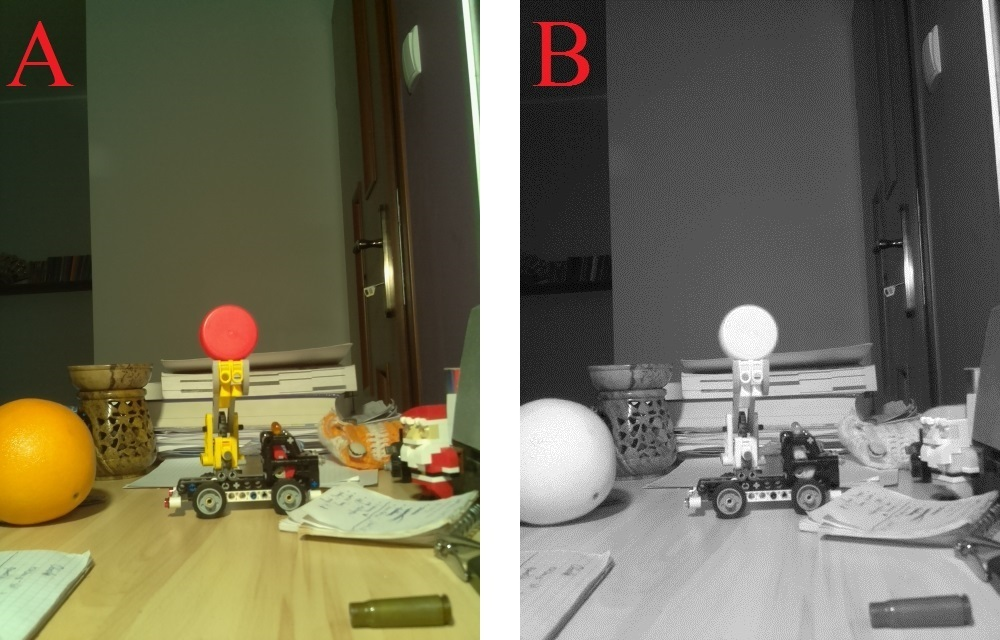
\includegraphics[scale=0.42]{imgs/imgBase+Red.jpg}
\caption[Uzyskany kanał czerwony wraz z oryginalny obrazem.]\small{"A" - oryginalne zdjęcie wykonane przez kamerę Raspberry Pi, "B" - kanał czerwony tego zdjęcia.}
\label{red}
\end{center}
\end{figure}
Analizując jedynie prawe zdjęcie, przedstawiające intensywność koloru czerwonego, nie sposób oddzielić barwy czerwonej od tych, w których skład wchodzi kolor czerwony. Konieczna jest dalsze przetwarzanie danego obrazu.

W przedstawianym algorytmie zdecydowano się na wyszczególnienie obiektów o kolorze czerwonym poprzez usunięcie z kanału czerwonego barw, w których czerwień jest tylko mniej istotną składową. Dokonanie tego poprzez proste odjęcie od barwy czerwonej barw zielonej oraz niebieskiej powoduje jednak zbyt duże podkreślenie różnic między obszarami o różnym oświetleniu. Sytuację taką prezentuje ilustracja \ref{red-b+g}. Widać na niej, że nawet na jednorodnych obiektach powstają bardzo duże różnice w jasności, zależne od padającego na obiekt światła.\newpage
\begin{figure}[H]
\begin{center}
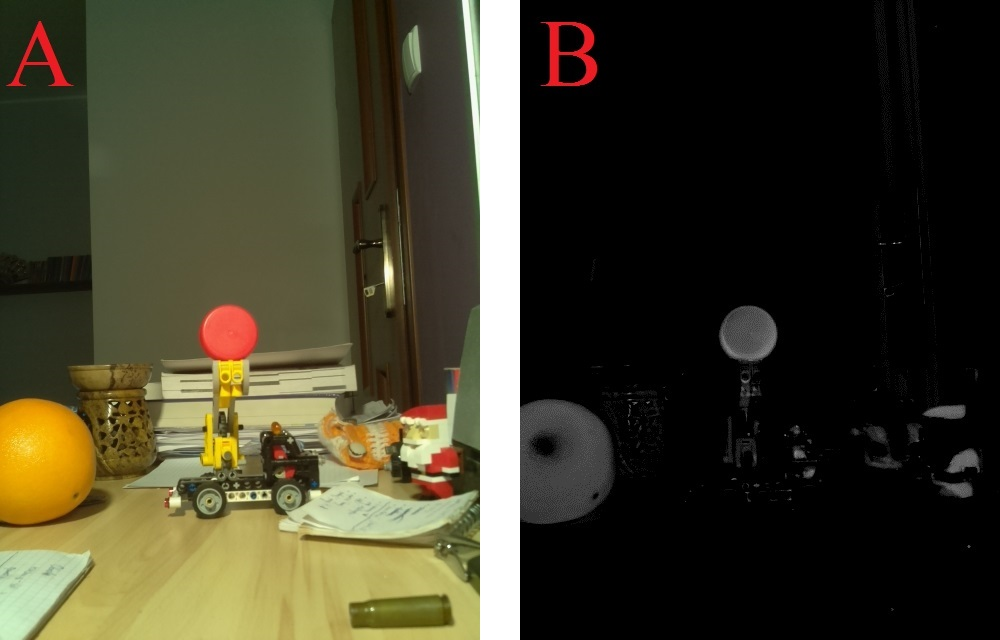
\includegraphics[scale=0.42]{imgs/imgBase+sumBG.jpg}
\caption[Kanał czerwony minus zielony oraz niebieski.]\small{"A" - przedstawiony dla porównania oryginalny obraz, "B" - obraz powstały z odjęcia od kanału czerwone sumy kanałów zielonego oraz niebieskiego.}
\label{red-b+g}
\end{center}
\end{figure}
Sytuacja taka może prowadzić do wielu nieprawidłowości w zachowaniu algorytmu, więc należało zastosować inną metodę wyszczególniania czerwonej barwy. Zamiast odejmowania sumy kanałów zielonego i niebieskiego zdecydowano się na wyznaczanie macierzy wartości maksymalnej tych dwóch barw i odejmowanie dopiero jej od kanału czerwonego. Operacja taka powoduje dużo mniejsze zróżnicowanie obrazu końcowego, który jest także mniej wrażliwy na zróżnicowane oświetlenie. Wynik operacji wyznaczającej maksimum kanału zielonego i niebieskiego oraz odjęcie go od kanału czerwonego przedstawia ilustracja \ref{red-max}.\newpage
\begin{figure}[H]
\begin{center}
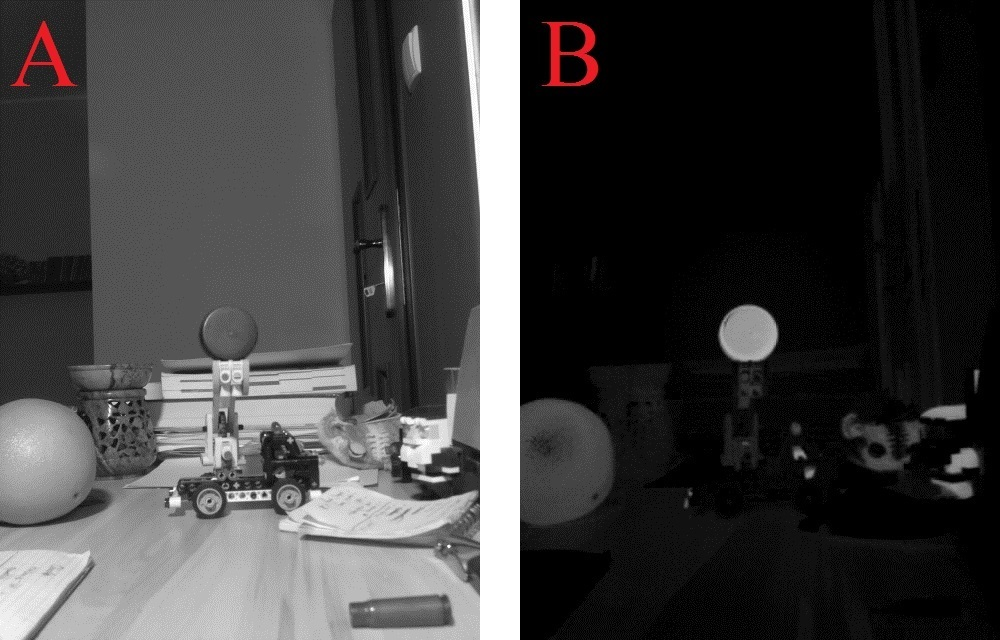
\includegraphics[scale=0.42]{imgs/imgMax+RwoBG.jpg}
\caption[Kanał czerwony minus maksimum zielonego i niebieskiego.]\small{"A" - obraz powstały jako maksimum kanałów zielonego i niebieskiego, "B" - wynik odjęcia wspomnianego maksimum od kanału czerwonego.}
\label{red-max}
\end{center}
\end{figure}
Jak widać poza bardziej jednolitym przedstawieniem jednorodnych obiektów udało się uzyskać bardziej wyróżniający się kolor czerwony w stosunku do np. pomarańczowego.

Odejmowanie od siebie zróżnicowanych obrazów powoduje jednak powstanie duże zróżnicowania jasności pikseli na niewielkiej odległości.  Efekt ten powoduje na dalszych etapach analizy obrazu problemy z odnajdywaniem regularnych geometrycznych kształtów, co sprowadza się do trudności z wykrywaniem, w szczególności niewielkich, okręgów. Problem ten rozwiązuje zastosowanie filtru medianowego na macierzy maksimów koloru niebieskiego i zielonego.

Filtr medianowy jest narzędziem wykorzystujący jedną z podstawowych wartości statystycznych jaką jest mediana. Polega ona na wyznaczaniu środkowego elementu w monotoniczne uporządkowanym ciągu\cite{Malina}. W przypadku filtru medianowego ciągiem tym jest zbiór pikseli, który na obrazie pokrywa maska filtru. Przykłady stosowanych masek przedstawia ilustracja \ref{maski}. Element środkowy, zaznaczony na niej jako "X", jest elementem do którego wpisany zostanie wynik mediany.\newpage
\begin{figure}[H]
\begin{center}
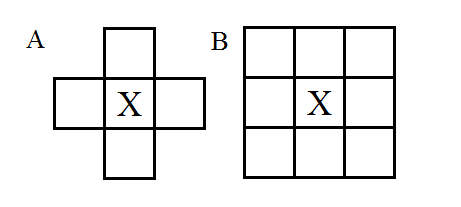
\includegraphics[scale=0.8]{imgs/maski.png}
\caption[Przykład masek filtru medianowego.]\small{Przykład masek wykorzystywanych w filtrze medianowym: a) maska 5-elementowa, b) maska 9-elementowa. Znakiem "X" oznaczono element środkowy.}
\label{maski}
\end{center}
\end{figure}
Filtr ten ujednolica obraz, usuwając z niego piksele o wartościach skrajnych. Ponadto jest cechą charakterystyczną jest także to, iż zaokrągla ona znajdujące się na obrazie kształty. Obie te cechy czynią z tego filtru narzędzie bardzo pożądanego w przedstawianym algorytmie, gdyż wyrównują one poszukiwane geometryczne regularności na obrazie, które wskutek przekształceń oraz niewielkiej rozdzielczości mogą zostać zniekształcone. Wykorzystywana w tym miejscy algorytmu maska ma kształt kwadratu oraz wymiary 5 na 5 pikseli. Efekt jej działania przedstawia ilustracja \ref{red-maxM}, na której widać obraz będący maksimum kanału zielonego i niebieskiego po dokonanej filtracji medianowej oraz wynik odejmowania od kanału czerwonego wspomnianego maksimum. Są to więc te same obrazy co na ilustracji \ref{red-maxM}, różniące się jedynie zastosowaniem filtracji.
\begin{figure}[H]
\begin{center}
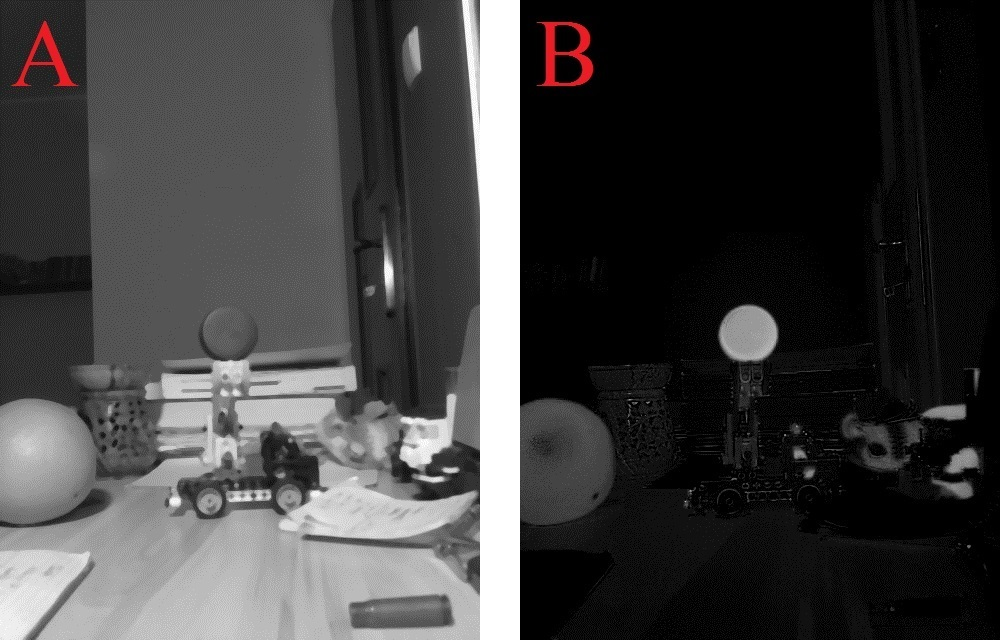
\includegraphics[scale=0.42]{imgs/imgMax+RwoBG_med.jpg}
\caption[Kanał czerwony minus maksimum zielonego i niebieskiego z filtrem medianowym.]\small{"A" - obraz powstały jako maksimum kanałów zielonego i niebieskiego oraz z filtrem medianowym, "B" - wynik odjęcia wspomnianego maksimum od kanału czerwonego.}
\label{red-maxM}
\end{center}
\end{figure}
Porównując obrazy "B" z ilustracji \ref{red-max} i \ref{red-maxM} widać oczekiwany efekt działania filtru. Krawędzie są bardziej dokładnie, a same obiekty posiadają bardziej jednolity poziom jasności.

Na tym etapie udało się uzyskać obraz z wyróżnionymi obszarami czerwonego koloru oraz o dużym poziomie szczegółowości. Kolejny etap algorytmu zakłada dokonanie segmentacji przetwarzanego obrazu. Segmentacja polega na podzieleniu obrazu na obszary, posiadające pewną cechą wyróżniające je od sąsiedztwa\cite{Malina}. W przedstawianym przypadku cechą tą jest posiadanie barwy czerwonej. Jedną z najprostszych metod segmentacji, wykorzystaną także w tym przypadku, jest progowanie. Polega ono na porównaniu każdego piksela z pewną wartością progową i w zależności od wyniku porównania przypisaniu mu jednej z dwóch wartości. Zasadę tą można przedstawić za pomocą wzoru \ref{progowanie}.
\begin{equation}
J_p(x, y) =
  \begin{cases}
    0	& \quad \text{dla } J(x, y) < t\\
    1	& \quad \text{dla } J(x, y) \geq t\\
  \end{cases}
\label{eq:progowanie}
\end{equation}
gdzie:
\begin{equationDescriptor}
\EQDitem{$J_p(x, y)$}{wartość piksela po progowaniu,}
\EQDitem{$J(x, y)$}{wartość piksela przed progowaniem,}
\EQDitem{$t$}{wybrany próg.}
\end{equationDescriptor}
Do przeprowadzenia progowania wykorzystana zostanie funkcja \texttt{threshold(InputArray src, OutputArray dst, double thresh, double maxval, int type)} z biblioteki \textit{OpenCV}. Dwa pierwsze argumenty, które są jej przekazywane to obraz wejściowy oraz wyjściowy. Kolejny, nazwany \texttt{thresh} jest wartością progu, dla której ma być przeprowadzona operacja. W przedstawianym algorytmie wartość ta została uzależniona od jasności samego obrazu, aby uzyskać poprawne działanie algorytmie przy różnych rodzajach oświetlenia otoczenia robota. Zdecydowano się na wartość 0.75 z poziomu najjaśniejszego piksela występującego na obrazie, co jest wartością dobraną na podstawie obserwacji wykonanych w szeregu testów wykonanych na różnorodnych obrazach. Kolejnym wprowadzanym do funkcji argumentem jest \texttt{maxVal}, za którego pomocą można ustalić poziom jasności dla pikseli wcześniej omawiany próg. Przy tym użyciu zastosowano wartość 255, a więc maksymalną jasność dla obrazów 8-bitowych. Ostatnim wprowadzanym do funkcji argumentem jest typ progowania który ma być zastosowany z wykorzystaniem powyższych parametrów. Poza zastosowanym w algorytmie progowaniem binarnym istnieje możliwość odwróconego progowania binarnego (gdzie pikselom nieprzekraczającym progu przypisywana jest ustalona wartość maksymalna, a te przekraczające próg są zerowane) lub zastosowania któregoś z tych progowań jedynie dla wartości poniżej albo powyżej progu. Ostateczny kształt wywołanej funkcji przyjął więc formę:
\begin{lstlisting}
cvThreshold(new IplImage(redImage), thresholdedImage, 0.75*maxValue, 255,
	CV_THRESH_BINARY);
\end{lstlisting}

Operacja progowania wykonywana na obrazie z pełną skalą szarości, przy pomocy stałego progu, może jednak powodować utratę części geometrii. Przykładowo w sytuacji, gdy krawędź czerwonego okręgu znajduje się w cieniu względem jego pozostałej części to istnieje ryzyko odcięcia danej krawędzi w trakcie progowania. W omawianym programie przed takimi sytuacjami chroni ponowne wykorzystanie filtru medianowego. Wspomniane wcześniej efekty jego działania, tj. wygładzanie krawędzi oraz wyrównywanie poziomu jasności bardzo dobrze nadaje się do przygotowania obrazu do operacji progowania, które ma za zadanie zachować regularne, geometryczne kształty. Obraz po operacji progowania bez zastosowanego filtru medianowego oraz z jego wykorzystaniem przedstawia ilustracja \ref{threshold}.
\begin{figure}[H]
\begin{center}
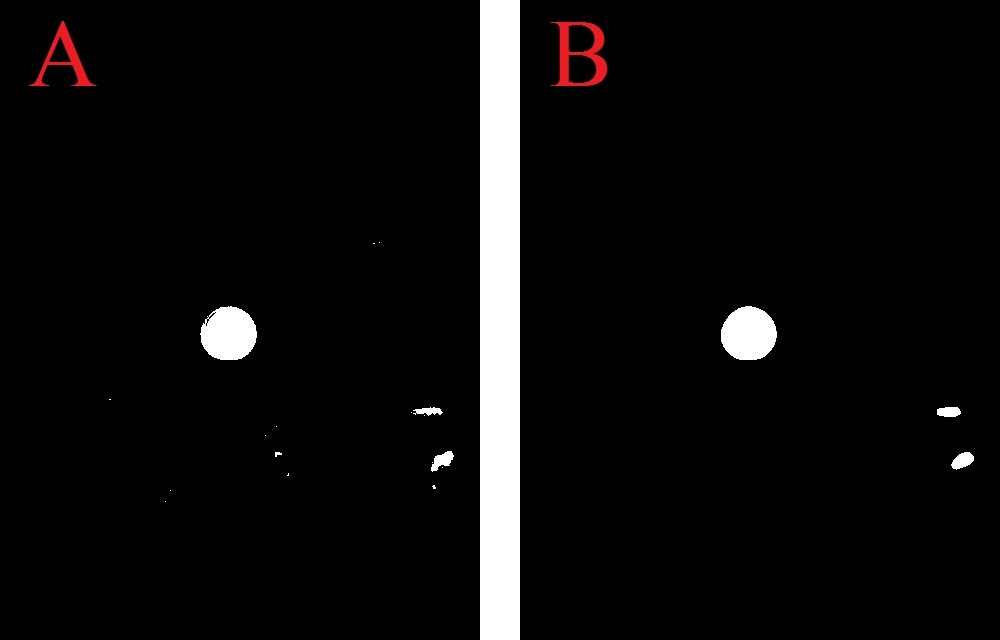
\includegraphics[scale=0.42]{imgs/threshold.jpg}
\caption[Efekt progowania z oraz bez filtru medianowego.]\small{"A" - obraz będący efektem progowania bez wcześniejszego zastosowania filtru medianowego, "B" - efekt operacji progowania po wcześniejszym zastosowaniu filtru medianowego.}
\label{threshold}
\end{center}
\end{figure}

\namedsection{Analiza obrazu}
Otrzymywany na wyjściu przetwarzania sprogowany obraz zostaje następnie poddany analizie, mającej za zadanie przeszukać go pod kątem występowania kół. Do tego celu wykorzystana została transformacja Hougha. Jej podstawowa wersja została opracowana przez Paula Hougha w 1962 roku i służyła do detekcji linii prostych. Z czasem metodę tę jednak rozwijano, uogólniając o inne dające się opisać analitycznie kształty. Jej wariacja służąca do detekcji okręgów została przedstawiona w 1972 przez Richarda Duda oraz Petera Harta.

Zasada działania algorytmu Hougha opiera się na budowie macierzy zwanej akumulatorem, której liczba wymiarów jest równa ilości zmiennych w funkcji szukanego obiektu. Każdy punkt tej macierzy odpowiada więc jednemu konkretnemu obiektowi znajdującemu się na obrazie. Wartość danej pozycji akumulatora jest inkrementowana dla każdego punktu na obrazie który może należeć do obiektu definiowanego przez tą pozycję. Po przeanalizowaniu w ten sposób całego obrazu wybiera się, zgodnie z założonym wcześniej progiem, maksima tego akumulatora, których współrzędne są parametrami znalezionych obiektów\cite{Sonka}.

Szukany okrąg możemy zdefiniować następującym wzorem:
\begin{equation}
(x - a)^2 + (y - b)^2 = r^2
\label{eq:kolo}
\end{equation}
gdzie:
\begin{equationDescriptor}
\EQDitem{$a, b$}{współrzędne środka okręgu,}
\EQDitem{$r$}{promień okręgu.}
\end{equationDescriptor}
W takim wypadku akumulator będzie macierzą o trzech wymiarach, odpowiednio dla współrzędnej $a$, $b$ oraz $r$. Każdy piksel, należący do krawędzi na badanym obrazie, będzie powodował inkrementację w macierzy akumulatora dla takich współrzędnych $a$, $b$ i $r$, dla których okręg o środku w punkcie $(a, b)$ i promieniu $r$ przecina badany piksel.

W module \texttt{imgproc.hpp} znajduje się funkcja, przeznaczona do detekcji okręgów za pomocą transformacji Hougha. Jej deklaracja przedstawia się w następujący sposób: \texttt{void cv::HoughCircles (InputArray image, OutputArray circles, int method, double dp, double minDist, \\double param1 = 100, double param2 = 100, int minRadius = 0, int maxRadius = 0)}.

Opis poszczególnych argumentów przedstawia się następująco:
\begin{itemize}
\item \texttt{image} - pierwszy z parametrów jest obrazem wejściowym, na którym przeprowadzana będzie analiza;
\item \texttt{circles} - drugim elementem na liście argumentów jest wyjściowy wektor znalezionych okręgów, każdy jego element zawiera współrzędne środka okręgu oraz jego promień;
\item \texttt{method} - definiuje metodę algorytmu, jednak w tym momencie jest dostępna tylko jedna - \textit{2-1 Hough Transform (21HT)}. Jest to metoda polegająca na rozbiciu całej operacji na dwa etapy z wykorzystaniem faktu, iż środek okręgu leży na każdej normalnej należącej do jego krawędzi. Pierwszy z etapów polega na uzupełnieniu dwuwymiarowego akumulatora danymi o normalnych przechodzących przez każdy punkt krawędzi obrazu. Na tej podstawie możliwe jest wyznaczenie szeregu potencjalnych środków okręgów jako punktów, w których przecina się znaczna ilość normalnych. Drugim etapem tej metody jest stworzenie histogramu z odległościami punktów brzegowych obrazu do wszystkich potencjalnych środków okręgów. Lokalne maksima na histogramie wskazują występowanie okręgów.\cite{Yuen}. Metoda ta jest stosowana ze względu to znaczne uproszczenie obliczeniowe: zamiast macierzy 3-wymiarowej stosowana jest 2-wymiarowa oraz histogram;
\item \texttt{dp} - następnym wprowadzanym do funkcji argumentem jest odwrócony stosunek rozmiaru akumulatora do oryginalnego obrazu. W przedstawianym programie, po przeprowadzeniu testów, zdecydowano się na wysoką wartość tego parametru, równą 2.3, gdyż ograniczona rozdzielczość oraz część szumów wynikających z przeprowadzanych operacji mogą prowadzić do pogorszenia regularności krawędzi obiektów, co właśnie jest niwelowane właśnie przez mniejszy akumulator. Dzieje się tak, gdyż mniejszy akumulator oznacza mniejszą ilość wartości  zmiennych między jakie dysponowane będą punkty krawędziowe obrazu;
\item \texttt{minDist} - kolejny argument odpowiada za minimalny dystans jaki może dzielić dwa wykryte okręgi;
\item \texttt{param1} - parametr odpowiedzialny wartość progu w algorytmie wykrywania krawędzi stosowanym przed transformatą Hougha. Jest on konieczny, gdyż zaimplementowana wersja Hougha operuje właśnie na mapie krawędzi. W omawianym programie parametr ten nie ma znaczenia, gdyż progowanie jest już przeprowadzane na obrazie binarnym;
\item \texttt{param2} - w tym miejscu ustalany jest próg selekcji środków okręgów wykrytych w pierwszej fazie transformaty Hougha \textit{21HT}. Ustawienie progu na wartość 100 oznacza, że wykryte zostaną jedyne pełne okręgi, posiadające wszystkie punkty brzegowe. Sukcesywne zmniejszanie tej wartości pozwala odnajdywać niepełne okręgi, częściowo zasłonięte, zniekształcone lub w sposób fałszywy interpretować krzywizny jako okręgi;
\item \texttt{minRadius, maxRadius} - ostatnie dwa parametry w tej funkcji decydują o maksymalnym oraz minimalnym rozmiarze okręgu, który ma być wykrywany przez algorytm. Pozostawienie obu tych wartości na zero sprawi, że ograniczenie takie nie będzie stosowane.
\end{itemize}

Ostatecznie zaimplementowana wersja tej funkcji przyjęła postać:
\begin{lstlisting}
HoughCircles(thresholdedImage, circles, HOUGH_GRADIENT, 2.3, 10, 200, 80, 0, 0);
\end{lstlisting}

Ilustracja \ref{przyklady} przedstawia wykryte okręgi na używanym do tej pory przykładowym obrazie oraz dwóch innych zdjęciach zrobionych przy zróżnicowanym oświetleniu. Ostatnie, czwarte zdjęcie zostało sprawdzane pod kątem zachowania się algorytmu przy braku odpowiedniego obiektu w przypadku sztucznego oświetlenia przekolorowującego scenę. Algorytm w sposób prawidłowy nie wykrył fałszywych okręgów.\newpage
\begin{figure}[H]
\begin{center}
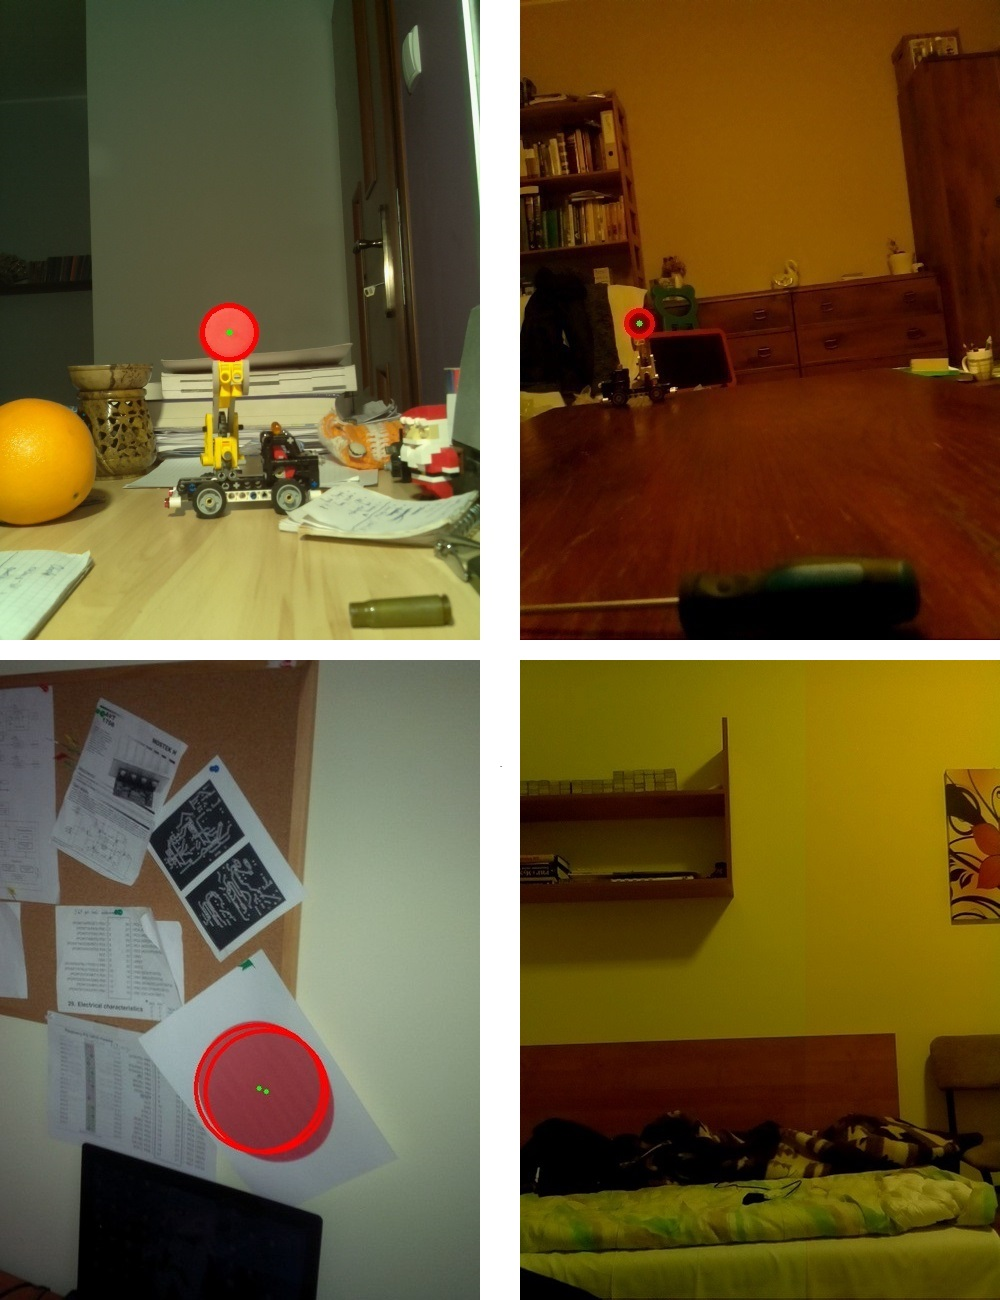
\includegraphics[scale=0.6]{imgs/circles.jpg}
\caption[Przykładowe efekty końcowe algorytmu wykrywającego okręgi.]\small{Ilustracja przedstawia trzy zdjęcia z czerwonymi obiektami wykonane w zróżnicowanym oświetleniu oraz jedno zdjęcie nie posiadające pożądanego obiektu, jednak przekolorowane sztucznym oświetleniem mogącym teoretycznie zmylić algorytm.}
\label{przyklady}
\end{center}
\end{figure}
